\documentclass[12pt, a4paper]{article}

% --- Pakiety ---
\usepackage[utf8]{inputenc}
\usepackage[T1]{fontenc}
\usepackage[polish]{babel}
\usepackage{amsmath, amssymb}
\usepackage{graphicx}
\usepackage{float}
\usepackage{geometry}
\usepackage{hyperref}
\usepackage{booktabs}
\usepackage{caption}
\usepackage{listings}
\usepackage{xcolor}
\usepackage{parskip}

\geometry{
  a4paper,
  left=2.5cm,
  right=2.5cm,
  top=2.5cm,
  bottom=2.5cm
}

\hypersetup{
  colorlinks=true,
  linkcolor=blue,
  urlcolor=blue
}

% --- Strona tytułowa ---
\title{
  \textbf{Metody Obliczeniowe w Nauce i Technice} \\[0.5em]
  \large Laboratorium 1 -- Analiza błędów
}
\author{Mateusz Stoch}
\date{18 marca 2026}

\begin{document}

\maketitle
\tableofcontents
\newpage

% ============================================================
\section{Zadanie 1 -- Numeryczne różniczkowanie}
% ============================================================

\subsection{Opis problemu}

Celem zadania jest numeryczne wyznaczenie pochodnej funkcji $f(x) = \tan(x)$ w punkcie $x_0 = 1$, przy użyciu dwóch schematów różnicowych: różnicy w~przód oraz różnicy centralnej. Analizowane są trzy składowe błędu obliczeniowego w~zależności od kroku $h$.

\subsection{Różnica w przód}

Pochodna funkcji jest przybliżana wzorem różnicy w~przód:
\begin{equation}
  f'(x) \approx \frac{f(x+h) - f(x)}{h}.
  \label{eq:forward}
\end{equation}

Całkowity błąd obliczeniowy $E(h)$ jest sumą dwóch niezależnych składowych:
\begin{itemize}
  \item \textbf{Błąd metody} (obcięcia) -- wynika z pominięcia wyrazów wyższego rzędu w~rozwinięciu Taylora. Dla różnicy w~przód:
    \begin{equation}
      E_{\text{metody}}(h) \approx \frac{|f''(x)|}{2}\, h.
      \label{eq:err_method_fwd}
    \end{equation}
  \item \textbf{Błąd numeryczny} (zaokrągleń) -- wynika z~ograniczonej precyzji reprezentacji liczb zmiennoprzecinkowych:
    \begin{equation}
      E_{\text{num}}(h) \approx \frac{2\,\varepsilon_{\text{mach}}\,|f(x)|}{h}.
      \label{eq:err_num_fwd}
    \end{equation}
\end{itemize}

Błąd obliczeniowy osiąga minimum w~punkcie, w~którym obie składowe są równe. Minimalizując $E(h) = E_{\text{metody}}(h) + E_{\text{num}}(h)$ względem $h$, otrzymuje się optymalny krok:
\begin{equation}
  h_{\min} \approx 2\sqrt{\frac{\varepsilon_{\text{mach}}}{|f''(x)|}}.
  \label{eq:hmin_fwd}
\end{equation}

Dokładna pochodna $\tan'(x)$ wyraża się jako:
\begin{equation}
  f'(x) = 1 + \tan^2(x).
\end{equation}

Druga pochodna, potrzebna do oszacowania błędu metody, wynosi:
\begin{equation}
  f''(x) = 2\tan(x)\bigl(1 + \tan^2(x)\bigr).
\end{equation}

\subsection{Różnica centralna}

Schemat różnicy centralnej jest dokładniejszy rzędu $O(h^2)$:
\begin{equation}
  f'(x) \approx \frac{f(x+h) - f(x-h)}{2h}.
  \label{eq:central}
\end{equation}

Składowe błędu wyglądają następująco:
\begin{itemize}
  \item \textbf{Błąd metody}:
    \begin{equation}
      E_{\text{metody}}(h) \approx \frac{|f'''(x)|}{6}\, h^2.
      \label{eq:err_method_cen}
    \end{equation}
  \item \textbf{Błąd numeryczny}:
    \begin{equation}
      E_{\text{num}}(h) \approx \frac{\varepsilon_{\text{mach}}\,|f(x)|}{h}.
      \label{eq:err_num_cen}
    \end{equation}
\end{itemize}

Optymalny krok dla różnicy centralnej:
\begin{equation}
  h_{\min} \approx \sqrt[3]{\frac{3\,\varepsilon_{\text{mach}}}{|f'''(x)|}}.
  \label{eq:hmin_cen}
\end{equation}

Trzecia pochodna, użyta w~powyższym wzorze:
\begin{equation}
  f'''(x) = 6\tan^4(x) + 8\tan^2(x) + 2.
\end{equation}

\subsection{Wyniki}

\begin{table}[H]
  \centering
  \caption{Zestawienie wartości $h_{\min}$ wyznaczonych empirycznie i~ze wzorów.}
  \begin{tabular}{lcc}
    \toprule
    Schemat & $h_{\min}$ empiryczne & $h_{\min}$ teoretyczne \\
    \midrule
    Różnica w przód   & $10^{-8}$ & $\approx 10^{-8}$ \\
    Różnica centralna & $10^{-7}$ & $\approx 10^{-7}$ \\
    \bottomrule
  \end{tabular}
  \label{tab:hmin}
\end{table}

Różnica centralna jest metodą rzędu wyższego, co przekłada się na mniejszy błąd obliczeniowy przy optymalnym $h_{\min}$. Wartość minimalna błędu $E(h_{\min})$ jest wyraźnie mniejsza dla schematu centralnego niż dla schematu w~przód.

\begin{figure}[H]
  \centering
  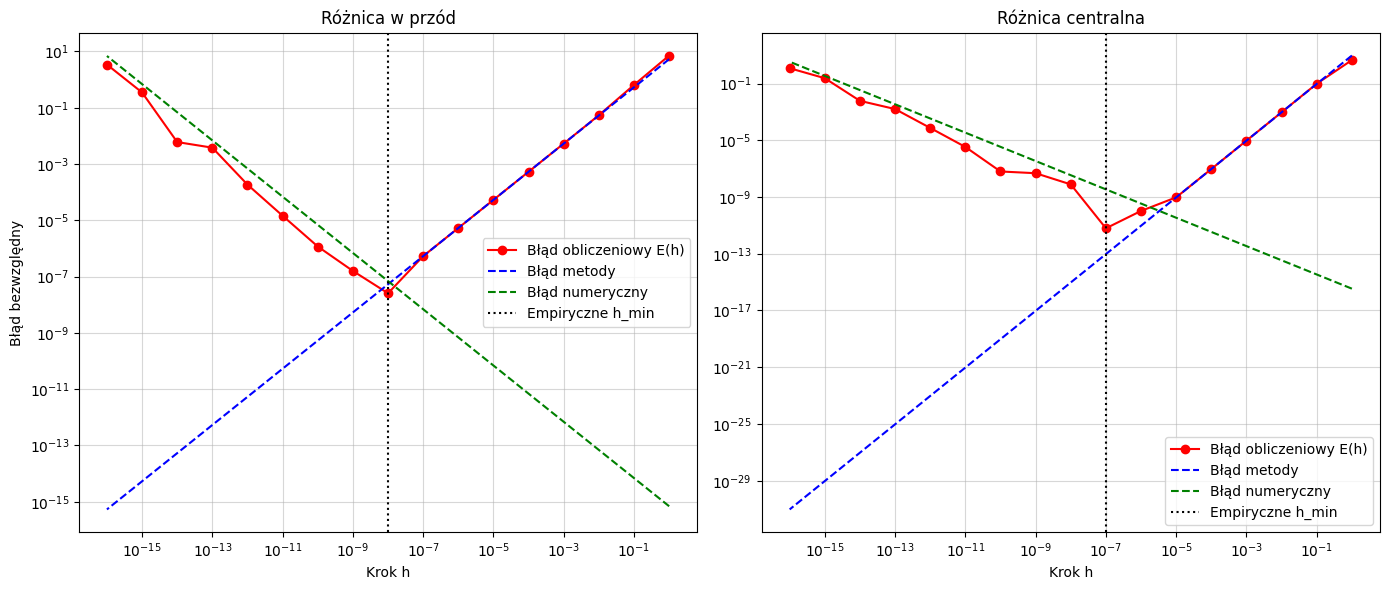
\includegraphics[width=\textwidth]{wykres1.png}
  \caption{Wykres 1. Składowe błędu numerycznego różniczkowania w~zależności od kroku $h$ (lewa strona -- różnica w~przód, prawa strona -- różnica centralna). Oś $x$ i~oś $y$ w~skali logarytmicznej.}
  \label{fig:wykres1}
\end{figure}

Na wykresie \ref{fig:wykres1} widoczne jest charakterystyczne minimum błędu obliczeniowego -- dla małych $h$ dominuje błąd zaokrąglenia (linia zielona), a~dla dużych $h$ dominuje błąd metody (linia niebieska). Pionowa linia przerywana oznacza empirycznie wyznaczone $h_{\min}$.

% ============================================================
\section{Zadanie 2 -- Numerycznie stabilne przekształcenia wyrażeń}
% ============================================================

\subsection{Opis problemu}

Niektóre wyrażenia matematyczne, choć poprawne analitycznie, mogą prowadzić do znacznych błędów numerycznych wskutek zjawiska \emph{katastrofalnego odejmowania} -- utraty cyfr znaczących podczas odejmowania dwóch bliskich sobie liczb. Poniżej przedstawiono stabilne numerycznie przekształcenia każdego z~wyrażeń.

\subsection{Przekształcenia}

\paragraph{(a) $\sqrt{x+1} - 1$ dla $x \approx 0$}

Dla małych $x$ obie liczby $\sqrt{x+1}$ i~$1$ są bliskie siebie, co powoduje utratę cyfr znaczących. Mnożąc i~dzieląc przez wyrażenie sprzężone, otrzymujemy:
\begin{equation}
  \sqrt{x+1} - 1 = \frac{(\sqrt{x+1}-1)(\sqrt{x+1}+1)}{\sqrt{x+1}+1} = \frac{x}{\sqrt{x+1}+1}.
\end{equation}

\paragraph{(b) $x^2 - y^2$ dla $x \approx y$}

Dla $x$ bliskiego $y$ różnica $x^2 - y^2$ jest obliczana jako różnica dwóch dużych, bliskich sobie liczb. Stabilna postać korzysta z~tożsamości algebraicznej:
\begin{equation}
  x^2 - y^2 = (x - y)(x + y).
\end{equation}

\paragraph{(c) $\dfrac{1 - \cos x}{\sin x}$ dla $x \approx 0$}

Gdy $x \to 0$, licznik $1 - \cos x \to 0$. Mnożąc licznik i~mianownik przez $(1 + \cos x)$ i~korzystając z~tożsamości $1 - \cos^2 x = \sin^2 x$:
\begin{equation}
  \frac{1 - \cos x}{\sin x} = \frac{(1 - \cos x)(1 + \cos x)}{\sin x (1 + \cos x)} = \frac{\sin^2 x}{\sin x (1 + \cos x)} = \frac{\sin x}{1 + \cos x} = \tan\frac{x}{2}.
\end{equation}

\paragraph{(d) $\sin x - \sin y$ dla $x \approx y$}

Stosując wzór na różnicę sinusów:
\begin{equation}
  \sin x - \sin y = 2\sin\!\left(\frac{x-y}{2}\right)\cos\!\left(\frac{x+y}{2}\right).
\end{equation}
Gdy $x \approx y$, wartość $\sin\!\left(\frac{x-y}{2}\right)$ jest obliczana bezpośrednio, co eliminuje utratę cyfr znaczących.

\paragraph{(e) $\dfrac{a+b}{2}$ -- środek odcinka $[a,b]$ (bisekcja)}

Dla liczb tego samego znaku może wystąpić przepełnienie lub błąd zaokrąglenia przy obliczaniu sumy $a+b$. Stabilna wersja to:
\begin{equation}
  \text{środek} = a + \frac{b - a}{2}.
\end{equation}

\paragraph{(f) $\operatorname{softmax}(x)_i = \dfrac{\exp(x_i)}{\sum_j \exp(x_j)}$}

Gdy elementy wektora $x$ są duże, wartości $\exp(x_i)$ mogą przekroczyć zakres reprezentacji liczb zmiennoprzecinkowych (overflow). Korzystając z~własności:
\begin{equation}
  \operatorname{softmax}(x)_i = \frac{\exp(x_i - c)}{\sum_j \exp(x_j - c)},
\end{equation}
gdzie $c = \max_j x_j$, unika się przepełnienia. Wynik jest matematycznie równoważny wersji oryginalnej, ponieważ stała $c$ skraca się w~liczniku i~mianowniku.

\subsection{Weryfikacja numeryczna}

Dla podpunktów (a) i~(b) weryfikację przeprowadzono przy użyciu biblioteki \texttt{decimal} z~precyzją 5 cyfr znaczących (\texttt{getcontext().prec = 5}).

\textbf{Podpunkt (a):} Dla $x = 10^{-4}$:
\begin{itemize}
  \item wersja niestabilna: $\sqrt{10^{-4}+1} - 1 \approx 5.0 \times 10^{-5}$ (błąd zaokrąglenia widoczny),
  \item wersja stabilna: $\dfrac{10^{-4}}{\sqrt{10^{-4}+1}+1} \approx 4.9999 \times 10^{-5}$ (wynik dokładniejszy).
\end{itemize}

\textbf{Podpunkt (b):} Dla $x = 100.01$, $y = 100.00$:
\begin{itemize}
  \item wersja niestabilna: $x^2 - y^2 = 10002.0001 - 10000.0 = 2.0$ (utrata cyfr znaczących),
  \item wersja stabilna: $(x-y)(x+y) = 0.01 \times 200.01 = 2.001$ (wynik prawidłowy).
\end{itemize}

% ============================================================
\section{Zadanie 3 -- Numeryczne wyznaczanie granicy funkcji}
% ============================================================

\subsection{Opis problemu}

Rozważamy funkcję:
\begin{equation}
  f(x) =
  \begin{cases}
    1 & \text{dla } x = 0, \\
    \dfrac{e^x - 1}{x} & \text{dla } x \neq 0.
  \end{cases}
  \label{eq:f3}
\end{equation}

\subsection{Granica analityczna}

Z rozwinięcia funkcji $e^x$ w szereg Taylora:
\begin{equation}
  e^x = 1 + x + \frac{x^2}{2!} + \frac{x^3}{3!} + \cdots
\end{equation}
wynika:
\begin{equation}
  \frac{e^x - 1}{x} = 1 + \frac{x}{2} + \frac{x^2}{6} + \cdots \xrightarrow{x \to 0} 1.
\end{equation}
Zatem $\lim_{x \to 0} f(x) = 1$.

\subsection{Metody obliczania}

W zadaniu zaimplementowano i~porównano cztery podejścia:

\begin{enumerate}
  \item \textbf{Formuła oryginalna}: $f(x) = (e^x - 1)/x$ -- dla małych $x$ mianownik $e^x - 1$ podlega katastrofalnemu odejmowaniu.

  \item \textbf{Formuła przez $y$}: Podstawiając $y = e^x$, definiujemy:
    \begin{equation}
      f(x) =
      \begin{cases}
        1 & \text{dla } y = 1, \\
        \dfrac{y - 1}{\ln y} & \text{dla } y \neq 1.
      \end{cases}
    \end{equation}
    Ta postać jest matematycznie równoważna wersji oryginalnej i~daje lepsze wyniki dla umiarkowanie małych $x$.

  \item \textbf{Szereg Taylora}: Dla małych $x$ stosuje się przybliżenie:
    \begin{equation}
      f(x) \approx 1 + \frac{x}{2} + \frac{x^2}{6}.
      \label{eq:taylor3}
    \end{equation}
    Metoda jest dokładna, gdy $x$ jest wystarczająco małe.

  \item \textbf{Funkcja \texttt{expm1}}: Funkcja $\texttt{expm1}(x) = e^x - 1$ jest zaimplementowana numerycznie w~taki sposób, by unikać utraty cyfr znaczących dla małych $x$:
    \begin{equation}
      f(x) = \frac{\texttt{expm1}(x)}{x}.
    \end{equation}
\end{enumerate}

\subsection{Omówienie wyników}

\begin{figure}[H]
  \centering
  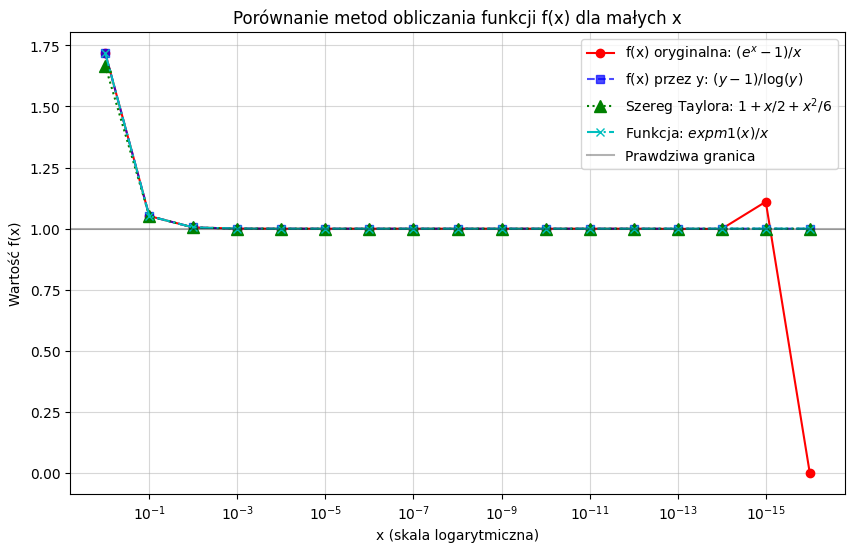
\includegraphics[width=0.85\textwidth]{wykres2.png}
  \caption{Wykres 2. Porównanie metod obliczania funkcji $f(x) = (e^x - 1)/x$ dla małych $x$.}
  \label{fig:wykres2}
\end{figure}

Na wykresie \ref{fig:wykres2} widać, że formuła oryginalna traci stabilność dla $x \lesssim 10^{-15}$, gdzie $e^x - 1$ jest zaokrąglane do zera, co skutkuje wynikiem $0/x = 0$ lub dzieleniem przez zero. Formuła przez $y$ poprawia zachowanie w~zakresie $10^{-14}$ do $10^{-2}$, jednak dla bardzo małych $x$ również traci dokładność. Szereg Taylora i~funkcja \texttt{expm1} zachowują wartość graniczną $f(x) \to 1$ na całym badanym przedziale, co czyni je metodami preferowanymi.

% ============================================================
\section{Zadanie 4 -- Sumowanie liczb zmiennoprzecinkowych}
% ============================================================

\subsection{Opis problemu}

Celem zadania jest porównanie pięciu metod sumowania $n$ liczb zmiennoprzecinkowych pojedynczej precyzji (\texttt{float32}), losowo wybranych z~rozkładu jednostajnego na przedziale $[0, 1]$. Jako wartość referencyjną przyjęto wynik funkcji \texttt{math.fsum}, która wykonuje sumowanie z~rozszerzoną precyzją.

\subsection{Metody sumowania}

\paragraph{(a) Podwójna precyzja (\texttt{float64})}

Sumowanie odbywa się sekwencyjnie w~porządku generowania, z~akumulatorem w~formacie \texttt{float64}. Zwiększona precyzja akumulatora znacząco redukuje błąd zaokrąglenia.

\paragraph{(b) Pojedyncza precyzja (\texttt{float32})}

Sumowanie sekwencyjne z~akumulatorem \texttt{float32}. Błąd zaokrąglenia kumuluje się przy każdym dodawaniu i~rośnie wraz z~$n$.

\paragraph{(c) Algorytm Kahana}

Algorytm sumowania z~kompensacją błędu, używający akumulatora \texttt{float32}:
\begin{align}
  &\text{sum} = 0, \quad \text{err} = 0 \notag \\
  &\text{for } i = 1, \ldots, n: \notag \\
  &\quad y = x_i - \text{err} \notag \\
  &\quad \text{temp} = \text{sum} + y \notag \\
  &\quad \text{err} = (\text{temp} - \text{sum}) - y \notag \\
  &\quad \text{sum} = \text{temp}
\end{align}
W każdym kroku śledzona jest utracona część $y$, która jest odejmowana w~kolejnej iteracji. Metoda osiąga błąd rzędu maszynowego niezależnie od $n$.

\paragraph{(d) Sumowanie rosnące}

Przed sumowaniem tablica jest sortowana rosnąco (od najmniejszych do największych wartości). Dodawanie liczb o~zbliżonej wielkości zmniejsza względny błąd zaokrąglenia.

\paragraph{(e) Sumowanie malejące}

Tablicę sortuje się malejąco (od największych do najmniejszych). Błąd jest większy niż przy sortowaniu rosnącym, ponieważ małe elementy są dodawane do już dużej sumy.

\subsection{Wyniki}

\begin{figure}[H]
  \centering
  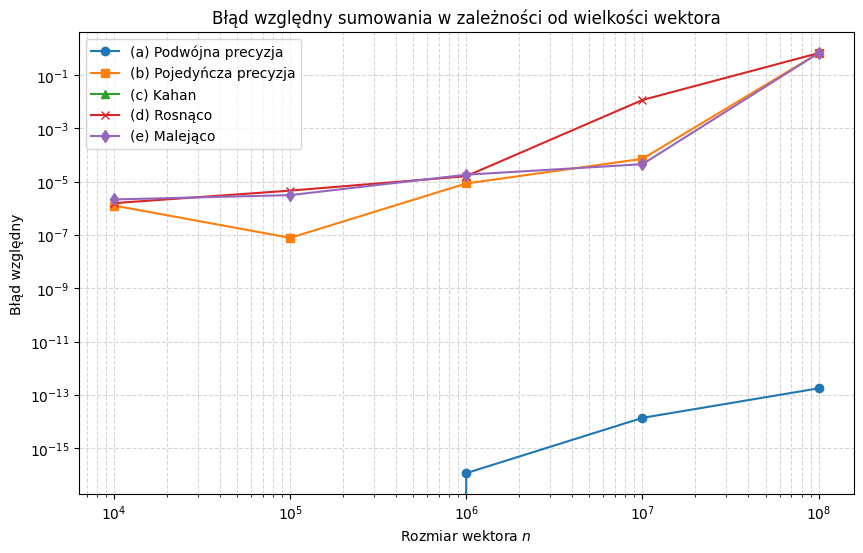
\includegraphics[width=0.9\textwidth]{wykres3.png}
  \caption{Wykres 3. Błąd względny sumowania w~zależności od $n$ (oś $x$ -- skala logarytmiczna, oś $y$ -- skala logarytmiczna).}
  \label{fig:wykres3}
\end{figure}

\begin{figure}[H]
  \centering
  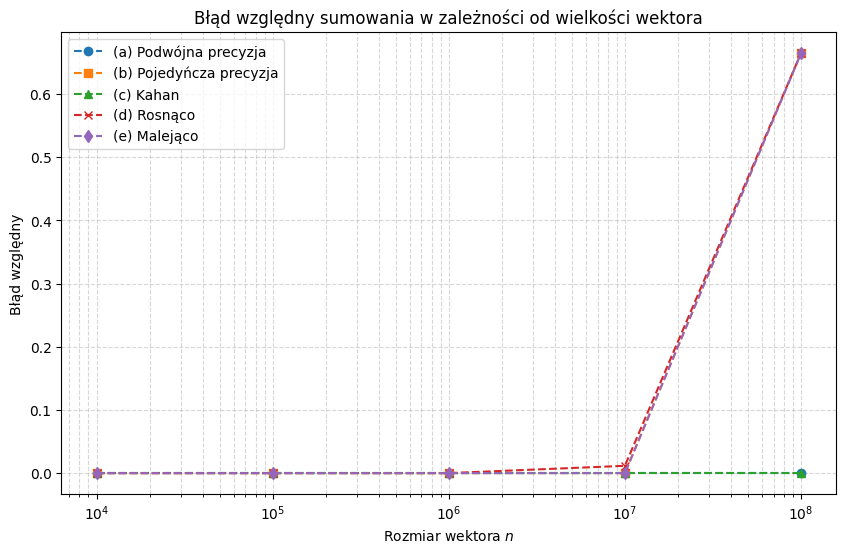
\includegraphics[width=0.9\textwidth]{wykres4.png}
  \caption{Wykres 4. Błąd względny sumowania w~zależności od $n$ (oś $x$ -- skala logarytmiczna, oś $y$ -- skala liniowa).}
  \label{fig:wykres4}
\end{figure}

\subsection{Omówienie wyników}

Z wykresów \ref{fig:wykres3} i~\ref{fig:wykres4} wynikają następujące obserwacje:

\begin{itemize}
  \item Metoda \textbf{(a) -- podwójna precyzja} osiąga zdecydowanie najmniejszy błąd względny, rzędu $10^{-13}$–$10^{-14}$. Jest to wynik użycia 64-bitowego akumulatora, który minimalizuje błąd zaokrąglenia przy każdym dodawaniu.
  \item Metoda \textbf{(b) -- pojedyncza precyzja} charakteryzuje się błędem rosnącym z~$n$, co jest typowym zachowaniem przy sekwencyjnym sumowaniu z~ograniczoną precyzją.
  \item Metoda \textbf{(c) -- algorytm Kahana} utrzymuje stały, mały błąd względny niezależnie od $n$. Efektywnie kompensuje błąd zaokrąglenia kosztem dodatkowych operacji arytmetycznych.
  \item Metody \textbf{(d) rosnąco} i~\textbf{(e) malejąco} dają zbliżone wyniki do metody (b), gdyż zasadniczo różnica polega jedynie na kolejności sumowania w~ramach tej samej precyzji.
  \item Na wykresie w~skali liniowej (Wykres 4) widoczny jest gwałtowny wzrost błędu metod (b), (d) i~(e) dla $n = 10^8$, podczas gdy metody (a) i~(c) pozostają w~pobliżu zera.
\end{itemize}

% ============================================================
\section{Wnioski}
% ============================================================

\begin{enumerate}
  \item Przy numerycznym różniczkowaniu istnieje optymalny krok $h_{\min}$, minimalizujący błąd obliczeniowy. Schemat różnicy centralnej jest dokładniejszy od schematu w~przód -- błąd metody maleje jak $O(h^2)$ zamiast $O(h)$, a~optymalny błąd obliczeniowy jest mniejszy.

  \item Algebraiczne przekształcenia wyrażeń mogą znacząco poprawić dokładność obliczeń numerycznych poprzez eliminację katastrofalnego odejmowania. Warto stosować je szczególnie wtedy, gdy argumenty funkcji są bliskie wartościom krytycznym.

  \item Dla funkcji o~granicy nieoznaczonej w~punkcie zainteresowania (np. $\lim_{x\to 0}(e^x-1)/x = 1$), formuła oryginalna może prowadzić do poważnych błędów numerycznych. Zastosowanie funkcji \texttt{expm1} lub rozwinięcia Taylora zapewnia poprawne wyniki.

  \item Spośród badanych metod sumowania najdokładniejsza jest metoda z~akumulatorem podwójnej precyzji oraz algorytm Kahana. Dla zastosowań wymagających wysokiej dokładności przy ograniczeniu do pojedynczej precyzji, algorytm Kahana stanowi efektywne rozwiązanie.
\end{enumerate}

\end{document}
